\chapter{Klassieke Mechanica}
\vspace{-1cm}\begin{flushright}
{\it `If I have seen further than others, \\ it is by standing upon the shoulders of giants'}\\ I. Newton
\end{flushright}
Voordat we de effecten van de relativiteitstheorie op de mechanica
bespreken geven we een korte samenvatting van de Klassieke
Mechanica. Tijdens het college wordt gebruik gemaakt van het boek
`Analytical Mechanics' van \newline Fowles \& Cassiday (7de editie). 
\section{Dynamica}
De ontdekking van de wetten van de dynamica was een dramatisch moment
in de geschiedenis van de wetenschap. Voordat Newton zijn Principia
publiceerde waren de bewegingen van planeten een mysterie.
Galilei maakte daarvoor al een
grote stap met zijn principe van relativiteit; de grote bijdrage van Newton  was
dat hij beschreef hoe voorwerpen {\it veranderen} van snelheid.
Hij formuleerde daartoe drie hoofdwetten van de
Mechanica. De Eerste Wet was een herhaling van het relativiteitsprincipe van Galilei.
De Tweede Wet gaf specifiek aan hoe de snelheid van een voorwerp
verandert als een uitwendige {\it kracht} hierop inwerkt, via
$\vec{F}=m\vec{a}$. Newton geeft hierbij niet aan hoe de kracht in het
algemeen verkregen wordt; maar hij maakt ons bewust van het feit dat
er krachten zijn\footnote{In \'e\'en geval geeft hij wel een
uitdrukking voor de kracht, namelijk voor de zwaartekracht. Newton
geeft aan dat de gravitationele aantrekkingskracht tussen twee
lichamen met massa's $m$ en $M$ langs de verbinding van de
zwaartepunten van de twee lichamen loopt en gelijk is aan
\[ F_z = G \frac{mM}{r^2} \]
waarbij $r$ de onderlinge afstand tussen de lichamen is en $G$ de
Newtonse constante, $G=6,673 \cdot 10^{-11} m^3 kg^{-1} s^{-2}$. Voor
de aantrekking op aarde benaderen we dit als $F_z = m g $ waarbij de
valversnelling is, $g=G M/R^2$, met $R$ de diameter van de aarde. De
valversnelling op aarde is gelijk aan $g=9,8$ ms$^{-2}$. },
waarmee we de dynamica van voorwerpen kunnen beschrijven. Hoewel een
aantal verschijnselen hiermee beschreven kunnen worden, zoals de
draaiing van de maan om de aarde, zijn veel problemen hiermee niet
exact op te lossen. Bijvoorbeeld de onderlinge gravitationele aantrekking van drie
hemellichamen. Ook kende Newton lang niet alle krachten, zoals hij zich bijvoorbeeld 
zeker niet bewust was van de inter-moleculaire krachten.

Maar hoewel hij niet alle krachten kende, had hij wel een algemeen
principe waar alle krachten aan moeten voldoen. Dit principe is vastgelegd in zijn
Derde Wet: {\it actie is -reactie}.  Het wil ongeveer zeggen:
stel dat we twee voorwerpen hebben waarbij de eerste een kracht
uitoefent op het tweede, en het daarbij een kant op duwt. Dan
zegt de Derde Wet dat er een kracht is dat deeltje 2 uitoefent
op deeltje 1, die het de tegenovergestelde kant uitduwt. En dit
principe geldt voor alle krachten en voor een willekeurige
hoeveelheid deeltjes.
\subsection{Behoud van impuls}
De consequentie van de Derde Wet van Newton is het volgende. Stel dat we twee deeltjes beschouwen, $A$ en $B$, die botsen volgens Newton, waarbij deeltje A een kracht uitoefent op $B$ gelijk aan: 
\[ \vec{F}=m\vec{a} = \frac{d}{dt} m\vec{v} = \frac{d}{dt} \vec{p} \]
met $\vec{p}=m\vec{v}$ de impuls. De Derde Wet zegt nu dat er een
tegengestelde kracht van deeltje $B$ op $A$ wordt uitgeoefend, die
tegengesteld is:
\begin{equation}
\frac{dp_A}{dt} = -\frac{dp_B}{dt} \;\;\;\; \rightarrow \;\;\;\; \frac{d}{dt}(p_A+p_B) = 0
\end{equation}
waarbij we de impulsen $p_A$ en $p_B$ hebben opgeteld. Maar nu concluderen we
 dat de verandering van de {\it totale} impuls nul is, met andere woorden: de totale impuls $p_A+p_B$ is
behouden bij de interactie: het is een getal dat constant is als functie van de tijd.

We kunnen over het algemeen de wet van behoud van impuls voor een gesloten systeem, waarbij er geen interactie met de buitenwereld is, schrijven als
\begin{equation}
\vec{p}_1 + \vec{p}_2 +\vec{p}_3 + \vec{p}_4 + \dots = constant 
\end{equation} 
Indien er wel een uitwendige kracht op het systeem werkt, $\vec{F}_{ext}$, geldt dus
\begin{equation}
\frac{d}{dt}\left(\vec{p}_1 + \vec{p}_2 +\vec{p}_3 + \vec{p}_4 + \dots \right) = \vec{F}_{ext}
\end{equation}
\subsection{Arbeid en vermogen}
Als we de kracht als functie van de tijd $t$ kennen, kunnen we de fundamentele vergelijking $\vec{F}=\frac{d\vec{p}}{dt}$ voor de vergelijking van de dynamica van het deeltje oplossen door te integreren:
\begin{equation}
\int_A^B d \vec{p} = \int_{t_A}^{t_B} \vec{F} dt  \;\;\;\; \mbox{oftewel:} \;\;\;\;
\vec{p}_A-\vec{p}_B = \int_{t_A}^{t^B} \vec{F} dt = \vec{S}
\end{equation} 
waarbij $\vec{p}_A$ de impuls op moment $t_A$ is en $\vec{p}_B$ de
impuls op moment $t_B$. De grootheid $\vec{S}$ wordt de {\it krachtstoot}
genoemd. Dit wil zeggen dat de impulsverandering van het deeltje
gelijk is aan de krachtstoot.

Bij de meeste problemen in de mechanica is echter de kracht niet
gegeven als functie van de tijd $t$, maar als functie van de plaats,
$\vec{F}(x,y,z)$. We kunnen dan de integraal pas doen als we $x$, $y$
en $z$ als functies van de tijd kennen, d.w.z. als we het probleem
opgelost hebben dat we proberen op te lossen! Om uit deze vicieuze
cirkel te ontkomen voeren we de begrippen {\it arbeid} en {\it
energie} in.

Daartoe beschouwen we een bewegend deeltje dat een kracht
ondervindt. De hoeveelheid {\it arbeid} die door de kracht gedurende de
verplaatsing over een afstandje $d\vec{r}$ wordt verricht, is gelijk aan
\begin{equation}
dA = \vec{F} \cdot d \vec{r} 
\end{equation}
Rechts staat het inproduct, dus arbeid is gelijk aan het product van
de verplaatsing met de component van de kracht in de richting van de
verplaatsing. De arbeid is nul als de kracht loodrecht op de
verplaatsing staat. De totale arbeid wordt verkregen door de 
infinitesimale gedeelten bij elkaar op te tellen; dit levert de integraal:
\begin{equation}
A = \int_A^B \vec{F} \cdot d\vec{r} 
\end{equation}
In veel praktische gevallen is de kracht constant, zowel in grootte
als in de richting. We zullen ons nu daartoe beperken.  In dit geval
kunnen we de kracht $\vec{F}$ `buiten het integraalteken' halen (het
is immers een constante) en de arbeid schrijven als
\begin{equation}
A = \int_A^B \vec{F} \cdot d\vec{r} = \vec{F}\cdot \int_A^B d \vec{r} = \vec{F} \cdot(\vec{r}_B-\vec{t}_A) 
\end{equation}
Hieruit volgt dat de arbeid in dit geval onafhankelijk is van het pad
of de route tussen de punten $A$ en $B$. We kunnen willekeurig welke
route kiezen om van $A$ naar $B$ te gaan, bij een constante kracht is
de verrichtte arbeid onafhankelijk van de gekozen weg. Deze krachten
worden {\it conservatieve krachten} genoemd.

Bij praktische toepassingen is het van belang te weten in welk tempo arbeid verricht wordt. Het {\it vermogen} op een bepaald moment wordt gedefinieerd door 
\begin{equation}\label{e:vermogen}
P = \frac{dA}{dt}
\end{equation}
en dit kunnen we ook schrijven als
\begin{equation}\label{e:vermogen2}
P = F \cdot \frac{d \vec{r}}{dt} = \vec{F} \cdot \vec{v}
\end{equation}

We kunnen nu het verband bepalen tussen de arbeid en de energie. We
vullen hiervoor de uitdrukking $\vec{F} = m\vec{a}=md^2 \vec{r} /dt^2$ in voor de arbeid:
\begin{eqnarray}\label{e:arbeid}
A &=& \int_A^B \vec{F} \cdot d\vec{r} = \int_{t_A}^{t_B} \vec{F} \frac{d \vec{r}}{dt} dt =
\int_{t_A}^{t_B} m\frac{d^2\vec{r}}{dt^2} \frac{d \vec{r}}{dt} dt \\ \nonumber
& = &
\int_{t_A}^{t_B} \frac{d}{dt} \left[ \frac{1}{2} m\left( \frac{d r}{dt}\right)^2\right] dt =
\frac{1}{2} m\vec{v}_B^2 - \frac{1}{2}m\vec{v}_A^2
\end{eqnarray}
Deze uitkomst betekent dat de arbeid $A$ altijd gelijk is aan het verschil van de grootheid $\frac{1}{2}mv^2$
aan het einde en het begin van de baan. Dit wordt de kinetische energie genoemd, en aangeduid door $T$:
\begin{equation}
T=\frac{1}{2} m v^2 \;\;\;\; \mbox{of} \;\;\;\; T = \frac{p^2}{2m}
\end{equation}
De arbeid, verricht op een deeltje, is gelijk aan de verandering van
van kinetische energie van dit deeltje.

\subsection{Potenti\"ele energie}
We zagen dat een kracht conservatief heet als de arbeid die verricht
wordt onafhankelijk is van de afgelegde route. In dat geval kan de
arbeid worden uitgedrukt als het verschil tussen een grootheid
$U(x,y,z)$, berekend in het begin- en eindpunt. Deze grootheid
$U(x,y,z)$ wordt de potenti\"ele energie genoemd en is een functie van
de co\"ordinaten van een deeltje. Als $\vec{F}$ een conservatieve kracht
is geldt dus
\begin{equation}\label{e:pot}
A = \int_A^B \vec{F} \cdot d\vec{r} = U_A - U_B
\end{equation}
oftewel: de potenti\"ele energie is een functie zodanig dat de
verandering tussen begin- en eindpunt gelijk is aan de arbeid die op
het deeltje verricht moet worden om het van het begin- naar het
eindpunt te laten bewegen.
We hebben voor kleine afstanden $d\vec{r}$ dus voor de potenti\"ele energie
\begin{equation}
\vec{F} \cdot d\vec{r} = -d U 
\end{equation}
omdat we zo de definitie van de potenti\"ele energie weer terug vinden bij integratie:
\begin{equation}
A=\int_A^B \vec{F}\cdot d\vec{r} = -\int_A^B dU = -(U_B-U_A) = U_A-U_B
\end{equation}
We kunnen deze vergelijking schrijven als 
\begin{equation}
\vec{F} = -\vec{\nabla} U 
\end{equation}
waarbij de {\it gradi\"ent} $\vec{\nabla}$ de richtingsafgeleide is. De gradi\"ent is
zodanig gedefinieerd dat voor de $x$, $y$ en $z$ componenten van de kracht geldt dat:
\begin{equation}
F_x = -\frac{\partial U}{\partial x}, \;\;\;
F_y = -\frac{\partial U}{\partial y}, \;\;\;
F_z = -\frac{\partial U}{\partial z}
\end{equation} 
\subsection{Behoud van energie}
Als de kracht op een deeltje conservatief is, kunnen we vergelijking~\ref{e:pot}
combineren met~\ref{e:arbeid} en vinden dan dat $T_B-T_A = U_A-U_B$ oftewel:
\begin{equation}
(T+U)_A = (T+U)_B
\end{equation}
De grootheid $(T+U)$ wordt de {\it totale energie} van het deeltje genoemd en aangeduid met $W$, dus
\begin{equation}
W = T+U = \frac{1}{2} m v^2 + U(x,y,z)
\end{equation}
en er volgt dat als de krachten op een deeltje conservatief zijn, de
totale energie van dat deeltje behouden blijft, oftewel constant in de tijd is. De
totale energie wordt dus behouden. Voor een vrij vallend deeltje in een zwaartekrachtsveld bijvoorbeeld
geldt dat $U=mgh$ waarbij $h$ de hoogte van het deeltje is. Uit het
behoud van energie volgt
\begin{equation}
W = \frac{1}{2}m v^2 + mgh = constant
\end{equation}
Tot zover de zeer beknopte samenvatting van de Klassieke Mechanica.  

%
%\chapter{Relativistische mechanica}
%\section{Botsingen}
%We gaan nu terug naar de Speciale Relativiteitstheorie. We zullen allereerst een tweetal botsingen
%analyseren, waarbij we gebruik maken van de Lorentztransformaties. We zullen zien dat, indien we
%de behoudswetten willen handhaven samen met de Lorentztransformaties, we de definities van impuls 
%moeten aanpassen.
%\subsection{Elastische verstrooiing}
%We nemen allereerst aan dat de
%botsing 'perfect' is, dat wil zeggen dat geen energie verloren gaat
%in verwarming van de deeltjes en wrijving kan worden  verwaarloosd. Denk
%hierbij aan twee biljartballen op een perfect gladde biljarttafel. We
%noemen dit `elastische botsingen'. We nemen twee deeltjes die met
%snelheid $\vec{u}_1$ en $\vec{u}_2$ op elkaar afkomen en na de botsing
%een de snelheid $\vec{v}_1$ en $\vec{v}_2$ hebben. We schrijven het
%behoud van impuls op als:
%\begin{equation}
%\alpha_1\vec{u}_1 +\alpha_2 \vec{u}_2 = \alpha_3 \vec{v}_1 +\alpha_4 \vec{v}_2
%\end{equation} 
%waarbij in de Klassieke Mechanica we natuurlijk identificeren:
%\begin{eqnarray} 
%\alpha_1 & = & \alpha_3 \;\;\;\;\mbox{massa van deeltje 1} \\ 
%\alpha_2 & = & \alpha_4 \;\;\;\;\mbox{massa van deeltje 2} 
%\end{eqnarray}
%oftwel
%\[
%m_A\vec{u}_1 + m_B \vec{u}_2 = m_A\vec{v}_1' + m_B \vec{v}_2'  
%\]
%De massa $m$ noemen we de 'trage massa' van de deeltjes. In Figuur~\ref{f:bots} is deze botsing weergegeven. 
%\begin{figure}[ht] 
%\centering
%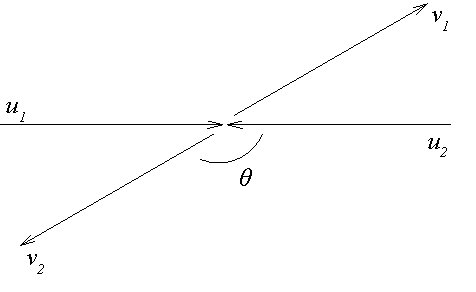
\includegraphics[width=.4\textwidth]{u1u2Horiz}
%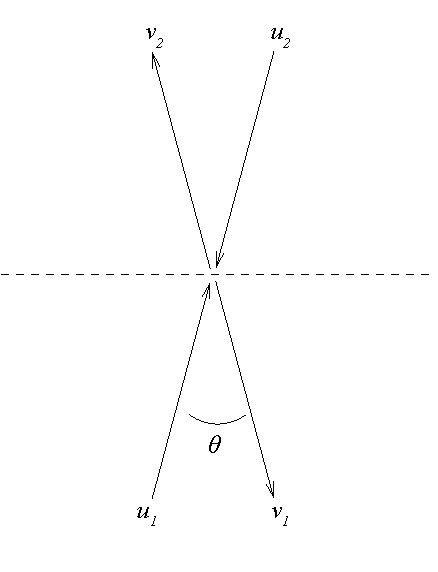
\includegraphics[width=.2\textwidth]{u1u2Vert}
%\caption{{\sl Elastische botsing tussen twee identieke deeltjes die met gelijke snelheid op elkaar worden afgeschoten. In het rechterfiguur is de botsing `gedraaid' zodat deeltje 1 van onderaf komt en deeltje 2 van bovenaf.\label{f:bots}}}
%\end{figure}
%In de relativiteitstheorie zullen we een extra snelheidsafhankelijke
%term toevoegen in de definitie van impuls. 
%
%De elastische botsingen tussen twee identieke deeltjes die met
%dezelfde grootte van snelheid $|\vec{u}|$ op elkaar af worden
%geschoten heeft
%$|\vec{u}_1|=|\vec{u}_2|=|\vec{v}_1|=|\vec{v}_2|$. Bij deze botsing
%wordt wel de richting van de deeltjes veranderd, en de inkomende en
%uitgaande deeltjes maken een hoek $\theta$
%
%
%We gaan nu deze botsing beschouwen vanuit een co\"ordinatenstelsel dat
%meebeweegt met deeltje 1. In dit stelsel heeft deeltje 1 geen snelheid in de
%$x$-richting, maar alleeen een snelheid in de $y$-richting. We noemen dit snelheid $w$.
%Deeltje 2
%maakt een hoek $\alpha$ met de $x$-as. Deze situatie is getekend in Figuur~\ref{f:bots2}.
%We hebben nu de situatie dat:
%\begin{itemize}
%\item Deeltje 1 gaat nu 'recht omhoog' met snelheid $w_1$ en terug met 
%snelheid $w_2$. Deze snelheden zijn aan elkaar gelijk maar tegengesteld. 
%\item Deeltje 2 heeft in dit stelsel een grotere snelheid
%$\vec{V}$. De $x$-component van de snelheid is $u$ en de $y$-component noteren we als $v$.
%\end{itemize}
%\begin{figure}[ht] 
%\centering
%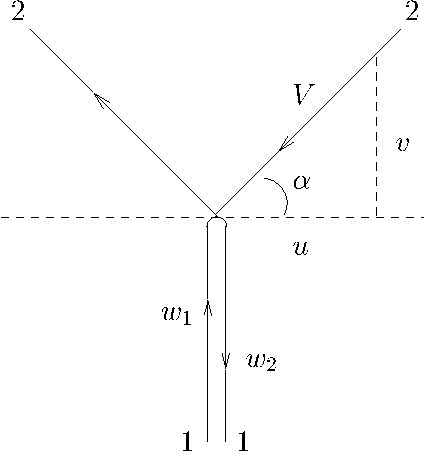
\includegraphics[width=.35\textwidth]{w1w2onder}
%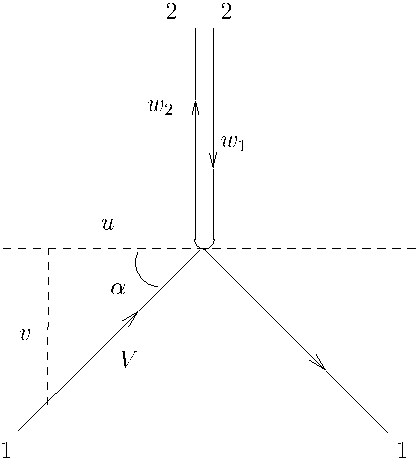
\includegraphics[width=.35\textwidth]{w1w2boven}
%\caption{{\sl Links: Botsing tussen twee identieke deeltjes in het stelsel dat meebeweegt met deeltje 1.
%Rechts: Botsing tussen twee identieke deeltjes in het stelsel dat meebeweegt met deeltje 2.
%\label{f:bots2}}}
%\end{figure}
%
%
%We vragen ons nu af of we een relatie tussen de $y$-componenten van de
%impuls van deeltje 1 en 2 kunnen vinden, dus een relatie tussen $w$ en
%$v$. Kijk hiervoor naar een ander stelsel $S'$ dat met deeltje 2
%meebeweegt. In $S'$ heeft deeltje 2 dus geen $x$-component van de
%snelheid, maar deeltje 1 wel. Uit symmetrie-everwegingen volgt dat de
%situatie nu precies gelijk is aan die in stelsel $S$, met deeltjes 1
%en 2 omgewisseld. Maar voor de transformatie van de snelheden in de
%$y$-richting hadden we uitdrukking~\ref{e:vy}, oftewel
%\begin{equation}
%V_y = \frac{V_y'}{\gamma}\frac{1}{1-\frac{\beta}{c}V'_x}
%\end{equation}
% Verder volgt
%\begin{eqnarray}
%V'_y & = & w \\
%V'_x & = & 0
%\end{eqnarray}
%met andere woorden: we hebben gevonden dat $v=w/\gamma$ (let op, $w$
%is de $y$-component van de snelheid van deeltje 1 in $S$, en van
%deeltje 2 in $S'$; $v$ is de $y$-component van deeltje 2 in $S$ en deeltje 1 in $S'$).
%Merk nu op dat:
%\begin{enumerate}
%\item De totale snelheid van bewegend deeltje 1 in $S$ en van bewegend deeltje 2 in $S'$ is hetzelfde, namelijk: $V=\sqrt{v^2+u^2}$.
%\item Impulsbehoud in de $y$-richting geeft nu
%\begin{equation}
%\alpha(w) w - \alpha(V) v = -\alpha(w) w + \alpha(V) v
%\end{equation}
%en let hierbij goed op het verschil tussen $V$ en $v$ en de tekens! We hebben nu
%\begin{equation}
%\frac{\alpha(V)}{\alpha(w)} = \frac{w}{v} = \frac{w}{w/\gamma} = \gamma \label{e:imprat}
%\end{equation}
%\end{enumerate}
%Neem nu de snelheid $w$ heel klein. In deze limiet is
%$\lim_{w\rightarrow 0} v = 0$ en $\lim_{w\rightarrow 0} V = u$. In dat
%geval kunnen we de relativistische effecten verwaarlozen en moeten we
%de Klassieke uitdrukking voor impuls terugvinden. Dit houdt in dat 
%\begin{equation}
%\lim_{w\rightarrow 0} \alpha(w) = m 
%\end{equation}
%en hiermee (invullen in~\ref{e:imprat}) vinden we
%\begin{equation}
%\lim_{w\rightarrow 0} \alpha(V) = \gamma m = \frac{m}{\sqrt{1-\frac{u^2}{c^2}}}
%\end{equation}
%We moeten dus de definitie van impuls aanpassen om te zorgen dat deze behouden blijft. Deze relativistische
%uitbreiding van impuls is
%\begin{equation}\label{e:impuls}
%\vec{p} = \gamma m \vec{v}
%\end{equation}
%Met deze definitie kunnen we de elastische botsingen relativistisch beschrijven. De factor $\gamma$ 
%is toegevoegd als gevolg van de transformatie van de snelheid in de $y$ richting.
%\subsection{Inelastische verstrooiing}
%We zullen nu een heel ander type botsingen beschouwen, namelijk de inelastische botsing. Hierbij 
%botsen twee deeltjes op elkaar zonder dat ze terugstoten. Denk nu aan twee klompen klei die
%op elkaar worden geschoten en na de botsing een grote klomp vormen. 
%
%\begin{figure}[ht] 
%\centering
%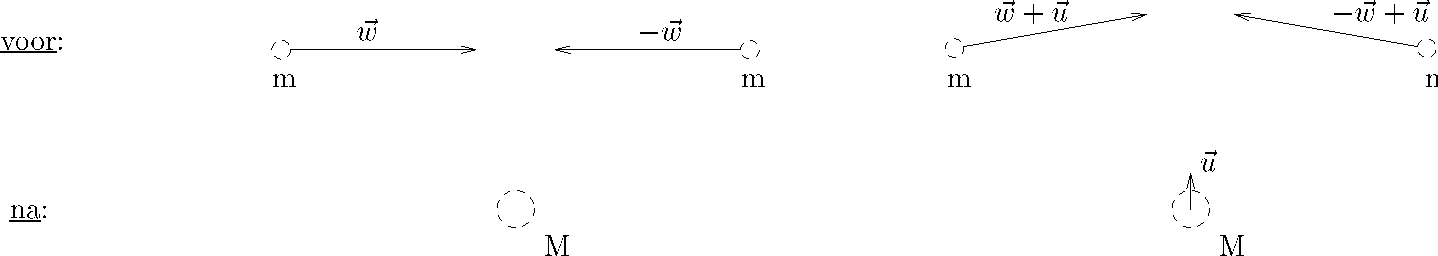
\includegraphics[width=.9\textwidth]{2mtotM}
%\caption{{\sl Links: Inelastische botsing tussen twee identieke deeltjes. Links in het stelsel waarin
%deeltje $M$ in rust is, rechts in het stelsel waarin $M$ een kleine snelheid $\vec{u}$ heeft. 
%Rechts: Botsing tussen twee identieke deeltjes in het stelsel dat meebeweegt met deeltje 2.
%\label{f:bots3}}}
%\end{figure}
%
%
%Neem twee identieke deeltjes met massa $m$ die een inelastische botsing maken. Beide komen met snelheid $w$ naar elkaar toe. Na de botsing is er \'e\'en stilstaand deeltje over met massa $M$. Klassiek verwachten
%we dat geldt $M=2m$.
%
%We beschouwen nu dezelfde botsing vanuit een stelsel dat met een kleine snelheid $u$ in de $y$-richting beweegt. De impuls voor en na de bosting in de $y$ richting levert:
%\begin{eqnarray}
%\mbox{voor} & p = & 2 \gamma m u \\
%\mbox{na}   & p = & M u 
%\end{eqnarray}
%waarbij we de relativistische definitie van de impuls hebben gebruikt, zie vergelijking~\ref{e:impuls}. We nemen weer de limiet $u\rightarrow 0$ en factor $\gamma$ staat dan voor $\gamma = 1/\sqrt{1-w^2/c^2}$.
%We hebben nu dus gevonden dat geldt:
%\begin{equation}
%M = 2\gamma m = \frac{2m}{\sqrt{1-\frac{w^2}{c^2}}}
%\end{equation}
%en dus is de massa $M$ na de botsing {\it groter} dan de som van de
%twee (rust-) massa's voor de botsing!  Dit is ook het gevolg van de
%wet van behoud van impuls. We zullen zien dat de toename van massa na
%de botsing afkomstig is van de kinetische energie v\`o\`or de botsing.
%\section{Relativistische energie}
%We geven eerst het gedachte experiment van Einstein waarin de
%gelijkheid van energie en massa werd gepostuleerd.  Dit
%gedachte-experiment is ook gepubliceerd in 1905, en is te vinden in de
%reader bij dit college. Vervolgens zullen we de energie van een bewegend voorwerp 
%beschouwen. 
%\subsection{De doos van Einstein}
%Als er \'e\'en natuurkundige wet is die iedereen kent, is dat wel de beroemde wet van equivalentie 
%tussen massa en energie
%\begin{equation}
%E= m c^2
%\end{equation}
%Einstein toonde deze wet eerst aan met een eenvoudig
%gedachteexperiment. In 1905 had hij eerst een verklaring voor het
%foto-elektrisch effect gegeven. Dit beschrijft het fenomeen waarbij
%licht op een plaatje valt en elektronen losmaakt. De energie van de
%elektronen bleek af te hangen van de `kleur' van het licht, en niet
%van de intensiteit van de lichtbron. De verklaring werd door Einstein
%gegeven door licht voor te stellen als deeltjes, fotonen, elk met een
%energie $E_{\gamma} = h \nu$. De constante $h$ is de constante van
%Planck en heeft de waarde $h=6.626\cdot 10^{-34} $kg m$^2$ s$^{-1}$, en
%$\nu$ staat voor de frequentie van het licht. De impuls van een foton
%is omgekeerd evenredig met de golflengte $\lambda$ en wordt gegeven
%door $p_{\gamma}=h/\lambda$. Met de uitdrukking $\lambda \nu = c$ is
%hiermee gegeven dat
%\[
%E_{\gamma} = c p_{\gamma}
%\]
%
%Het gedachte-experiment van Einstein (`Einsteins doos') gaat nu als
%volgt. Stel je een doos voor, volledig afgesloten van de
%buitenwereld. De doos heeft een massa $M$. Aan de linkerkant van de
%doos wordt nu een foton uitgestraald door de wand, en vertrekt naar de
%rechterkant van de doos. Op het moment van vertrek krijgt de doos een
%terugstoot van het vertrekkend foton. De impuls van het foton
%wordt gegeven door $p_{\gamma}=E/c$ en de impuls van de terugstoot
%door $p=Mv$. Met andere woorden, de snelheid van de doos, $v$, door de terugstoot is gelijk aan
%$v=-p/M = -E/ cM$. We hebben hier de klassieke benadering voor de impuls genomen.
%
%
%Op het moment dat het foton aan de andere kant aankomt wordt de
%terugstoot tenietgedaan en staat de doos weer stil. De doos is dan
%verplaatst over een afstand $\Delta x$. Deze afstand is gelijk aan $\Delta x=v \Delta t$,
%waarbij $\Delta t$ de tijd voorstelt die het foton er over doet om door de
%doos te vliegen, $\Delta t = L/c$ met $L$ de grootte van de doos.
%Hiermee is dus de afgelegde afstand $\Delta x=-vL/c = -EL/c^2 M$. 
%
%\begin{figure}[ht] 
%\centering
%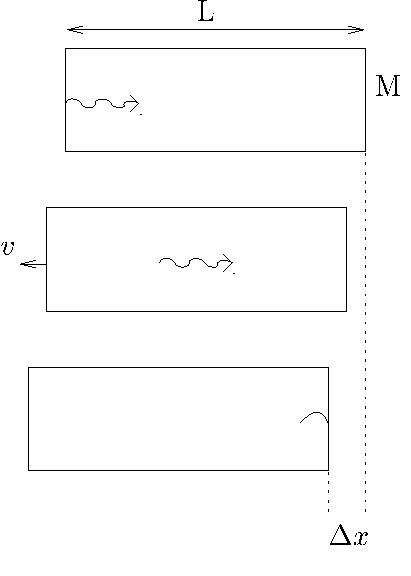
\includegraphics[width=.5\textwidth]{EinsteinBox}
%\caption{{\sl De `doos van Einstein'. Voor de uitleg zie tekst.
%\label{f:bots4}}}
%\end{figure}
%
%
%Het foton heeft pure energie getransporteerd; geen massa! Maar het
%zwaartepunt van de doos, dat geen kontakt met de buitenwereld heeft, kan door deze
%aktie van het foton niet verplaatst zijn. Als er een massa $m$ verplaatst zou zijn geweest, 
%over de lengte $L$ van de doos, zegt het behoud van het zwaartepunt:
%\[
%mL + M\Delta x = 0
%\]
%Nu kunnen we invullen voor $\Delta x$ en krijgen:
%\[
% mL - M\frac{EL}{c^2M} = 0\;\;\;\; \mbox{oftewel:} \;\;\;\; L\left(m-\frac{E}{c^2}\right) = 0
%\]
%en hiermee $E=mc^2$!
%
%Met andere woorden: de pure energie $E$ van het foton is equivalent aan een massa $m$ waarvoor geldt
%$m=E/c^2$. Het is aan Einstein te danken dat hij deze relatie algemeen heeft opgevat: energie is 
%gelijk aam massa.
%
%\subsection{Energie van een bewegend voorwerp}
%Met het gedachteexperiment heeft Einstein aangetoond dat energie en
%massa aan elkaar gelijk zijn via de relatie $E=mc^2$. Voor een
%voorwerp dat met een snelheid beweegt hebben we aangetoond dat de
%impuls wordt aangepast, en de relativistische beschrijving wordt
%gegeven door
%\begin{equation}\label{e:impulsmov}
%\vec{p} = \gamma m \vec{v}
%\end{equation} 
%Zo kunnen we ook postuleren dat de energie van het voorwerp gelijk is aan
%\begin{equation}\label{e:energymov}
%E = \gamma m c^2
%\end{equation} 
%en we zullen aantonen dat we met deze uitdrukking de juiste Klassieke Limiet verkregen wordt. 
%Immers, we kunnen voor lage snelheden benaderen dat
%\[
%\gamma  = \frac{1}{\sqrt{1-\frac{v^2}{c^2}}} \sim \left( 1 + \frac{v^2}{2c^2} - 
%\frac{3}{8}\frac{v^4}{c^4}\right)  
%\]
%en vinden dus dat
%\[
%E = \gamma m c^2 ~ mc^2 + \frac{1}{2} m v^2 - \frac{3}{8} m v^4 / c^2
%\]
%In de limiet voor lage snelheden is dit is precies de kinematische energie $\frac{1}{2}mv^2$ 
%plus een constante, $mc^2$. Energiebehoud wordt door dergelijke 
%constanten uiteraard netjes intact gelaten.
%
%We zullen nu ook laten zien dat deze definitie voor de energie,
%vergelijking~\ref{e:energymov}, overeenstemt met de klassieke relatie
%tussen energie en kracht, zoals gegeven in
%vergelijkingen~\ref{e:vermogen} en~\ref{e:vermogen2}. We hebben gezien dat verandering van energie
%$dE/dt$ teweeg wordt gebracht door het vermogen $\vec{F}\cdot \vec{v}$. Invullen levert:
%\begin{equation}
%\frac{dE}{dt} = \frac{d\gamma m c^2 }{dt} = \vec{v}\cdot \vec{F} = \vec{v} \cdot \frac{d\vec{p}}{dt}  = \vec{v}\frac{d\gamma m\vec{v}}{dt}
%\end{equation}
%We zullen nu laten zien dat deze vergelijking inderdaad consistent is. Daartoe vermenigvuldigen we met $2\gamma m$ om tot totale afgeleiden te komen:
%\begin{eqnarray}
%2\gamma m c^2 \frac{d\gamma m}{dt} = 2\gamma m \vec{v} \cdot \frac{d\gamma m \vec{v}}{dt} \\
%c^2 \frac{d}{dt} \left( \gamma m\right)^2 = \frac{d}{dt}\left( \gamma m v\right)^2
%\end{eqnarray}
%Hieruit volgt dat moet gelden:
%\[
%c^2 \gamma^2 m^2 = \gamma^2 m^2 v^2 +C
%\]
%waarbij $C$ een integratieconstante is, en het inproduct $\vec{v}\cdot \vec{v}$ geschreven wordt als $v^2$. Om de integratieconstante te bepalen vullen we snelheid $v=0$ in. Dan is $\gamma=1$ en volgt:
%\[
%c^2 m^2 = C
%\]
%zodat we kunnen schrijven
%\[
%c^2\gamma^2 m^2 - \gamma^2 m^2 v^2 = c^2 m^2
%\]
%waaruit we kunnen afleiden dan moet gelden dat 
%\[
%\gamma^2 = \frac{c^2}{c^2-v^2} = \frac{1}{1-\frac{v^2}{c^2}}
%\]
%hetgeen precies is wat we verwachten voor $\gamma$. Met andere woorden: de relativistische 
%uitdrukking voor de energie stemt overeen met de relaties tussen energie en kracht zoals gegeven door de Klassieke Mechanica.
%
%
%
%
%\section{Energie-impuls vector}
%We kunnen de relativistische uitdrukkingen voor energie en impuls ook
%op een ander manier benaderen. Daartoe keren we terug naar de
%vier-vectoren $x=(ct,x,y,z)$, en vragen ons af of er nog andere
%vier-vectoren te defini\"eren zijn.
%
%Daartoe laten we ons inspireren door de definitie van impuls in de Klassieke Mechanica: 
%\[
%\vec{p} = m\vec{v} = \lim_{\Delta t \rightarrow 0} m\frac{\Delta \vec{x}}{\Delta t}
%\]
%waarbij $\Delta x$ de verplaatsing in de $x$-richting is en $\Delta t$
%de tijdsduur. We vragen ons af of hier een equivalente vier-vector van
%te maken is in de vier-dimensionale ruimte-tijd. Dit is inderdaad
%mogelijk door $\Delta \vec{x}$ te vervangen door de viervector $\Delta x$.
%We kunnen echter niet $\Delta t$ in de noemer laten staan, omdat deze niet invariant onder de Lorentz
%transformaties is. We kunnen wel $\Delta t$ vervangen door het verloop van de eigentijd, $\Delta \tau$,
%omdat $\tau$ immers een scalar is. Als vier-vector kunnen we dus schrijven:
%\begin{equation}
%p =(p_0,p_1,p_2,p_3) =  \left( m\frac{c\Delta t}{\Delta \tau}, m \frac{\Delta x}{\Delta \tau}
%, m \frac{\Delta y}{\Delta \tau}, m \frac{\Delta z}{\Delta \tau}\right)
%\end{equation}
%en de vier-vector $p$ van  een voorwerp heeft nu de richting langs de wereldlijn van dit
%voorwerp in de ruimte-tijd. Voor de limiet $\Delta \tau\rightarrow 0$ kunnen we de componenten
%van de vier-vector identificeren als:
%\begin{eqnarray}
%p_0 & = & \frac{E}{c} \\
%p_1 & = & p_x \\
%p_2 & = & p_y \\
%p_3 & = & p_z 
%\end{eqnarray}
%immers, voor de componenten geldt:
%\begin{eqnarray}
%\frac{E}{c} & = & m c \frac{dt}{d\tau} = \gamma m c\\
%p_x & = & m \frac{dx}{d\tau} = \gamma mv_x \\
%p_y & = & m \frac{dy}{d\tau} = \gamma mv_y \\
%p_z & = & m \frac{dz}{d\tau} = \gamma mv_z 
%\end{eqnarray}
%Alle vier deze componenten zijn behouden bij een interaktie (d.w.z.
%botsing). De componenten zijn niet hetzelfde in elk stelsel $S$ of
%$S'$. Wel is de lengte van de vier-vector invariant, met andere
%woorden, de uitdrukking
%\begin{equation}
%\left(\frac{E}{c}\right)^2 - |\vec{p}|^2 
%\end{equation}
%is hetzelfde in elk stelsel. Deze uitdrukking is gelijk aan:
%\begin{eqnarray}\nonumber
%|p|^2 & = &  \left(\frac{E}{c}\right)^2 - |\vec{p}|^2  \\
%      & = & m^2c^2 \frac{dt^2}{d\tau^2}-m^2\frac{dx^2}{d\tau^2}-m^2\frac{dy^2}{d\tau^2}-m^2\frac{dz^2}{d\tau^2}\\ \nonumber
%      & = & m^2\frac{\left(d c^2 t^2 - dx^2 - dy^2 - dz^2\right)}{d\tau^2} \\ \nonumber
%      & = & m^2 c^2 \frac{d\tau^2}{d\tau^2} \\ \nonumber
%      & = & m^2 c^2
%\end{eqnarray}
%we kunnen dit schrijven als
%\begin{equation}
%E^2 - c^2 |\vec{p}|^2 = m^2 c^4
%\end{equation}
%en dit is de relativistische relatie tussen energie en impuls. Het is
%niets anders dan de lengte van de vier-vector $p$. Het `min'-teken is
%deze uitdrukking is hetzelfde `min'-teken als we al eerder zagen in de
%Minkowski-ruimte: dit maakte de ruimte-tijd fundamenteel anders dan de
%Euclidische ruimte.
%
%Merk verder op dat $m$ een invariante grootheid is, die hetzelfde is in alle stelsels. De uidrukking is
%overigens {\it kwadratisch} voor de energie, dus heeft de energie zelf twee oplossingen, namelijk $E=\pm 
%\sqrt{m^2 c^4 + c^2 |\vec{p}|^2}$. Dit zal uiteindelijk, wanneer het gecombineerd wordt met de quantummechanica, aanleiding geven tot het bestaan van anti-materie.
%
%De Lorentz-transformatie voor de componenten van de vier-vector $p$ kunnen verkregen worden door de componenten in te vullen. Het levert op voor een boost langs de $x$-as:
%\begin{eqnarray}
%\frac{E'}{c} &=& \gamma\left(\frac{E}{c} - \beta p_x \right) \\
%p_x' & = & \gamma\left( p_x - \beta \frac{e}{c}\right) \\
%p_y' & = & p_y \\
%p_z' & = & p_z
%\end{eqnarray}
%
%
%\subsection{Massaloze deeltjes}
%We zien dat de relativiteitstheorie massaloze deeltjes toelaat:
%\begin{displaymath}
%E = pc
%\end{displaymath}
%leidt tot
%\begin{displaymath}
%M = 0
%\end{displaymath}
%Aangezien uit formules \ref{e:impulsmov} en \ref{e:energymov} volgt dat
%\begin{displaymath}
%p = \frac{E}{c} \beta 
%\end{displaymath}
%(ga na) geldt voor massaloze deeltjes dus:
%\begin{displaymath}
%p = \frac{pc}{c} \beta = p \beta
%\end{displaymath}
%Hieruit volgt dat $\beta = 1$, dus $v = c$.
%M.a.w. massaloze deeltjes bewegen met de lichtsnelheid; zij kunnen niet stilstaan. Het foton
%is het bekendste voorbeeld. 
%
%\section{Samenvatting}
%De relativistische relatie tussen energie, impuls en snelheid kan worden samengevat als:
%\begin{eqnarray}
%E\leftrightarrow \vec{p} & \mbox{:} & E^2 - c^2 |\vec{p}|^2 = m^2 c^4 \\ \nonumber
%E\leftrightarrow \vec{v} & \mbox{:} & E = \gamma m c^2 \\ \nonumber
%\vec{p} \leftrightarrow \vec{v} & \mbox{:} & \vec{p} = \gamma m \vec{v} 
%\end{eqnarray}
%De relatie tussen de energie, impuls en snelheid wordt gegeven door:
%\begin{equation}
%\frac{c\vec{p}}{E} = \frac{\gamma m \vec{v} c}{\gamma m c^2} = \frac{\vec{v}}{c} = \vec{\beta}
%\end{equation}
%dus 
%\begin{equation}
%\vec{\beta} = \frac{\vec{v}}{c} = \frac{c\vec{p}}{E}
%\end{equation}
%
%\section{Enige opmerkingen n.a.v. botsingen} 
%
%In de beschrijving van een botsing tussen een willekeurig aantal
%deeltjes kunnen we nog het volgende opmerken. Bij de botsing
%zijn de {\it ingaande} deeltjes te onderscheiden van de {\it
%uitgaande} deeltjes. Voor een systeem van $n$ ingaande deeltjes en
%$m$ uitgaande deeltjes gelden de volgende behoudswetten:
%\begin{eqnarray}
%\sum_{deeltjes}^n p_x^{in} & = & \sum_{deeltjes}^m p_x^{uit} \\ \nonumber
%\sum_{deeltjes}^n p_y^{in} & = & \sum_{deeltjes}^m p_y^{uit} \\ \nonumber
%\sum_{deeltjes}^n p_z^{in} & = & \sum_{deeltjes}^m p_z^{uit} \\ \nonumber
%\sum_{deeltjes}^n E^{in} & = & \sum_{deeltjes}^m E^{uit}
%\end{eqnarray}
%Dit zijn de behoudswetten van de botsing: dat wil zeggen dat deze grootheden, impuls en energie, 
%voor en na de botsing hetzelfde zijn. Deze grootheden hangen af van het stelsel $S$ waarin we de botsing 
%beschouwen. De invariant $E^2-c^2|\vec{p}|^2$ is hetzelfde in elk co\"ordinatenstelsel $S$. Deze grootheid is ook behouden voor het hele systeem, maar niet voor elk deeltje afzonderlijk.
%
%De `massa van een systeem' leidt soms tot verwarring. Een lichaam met grote temperatuur heeft meer energie en 
%dus een grotere massa. Bijvoorbeeld, water van 40$^o$ C heeft een grotere massa dan water van 15$^o$ C. De toename in massa is ongeveer een fractie 10$^{-12}$. Maar wat neemt er nu eigenlijk toe? Niet de massa van de individuele
%molekulen. Het is de (bewegings) energie van het systeem van molekulen dat toeneemt.
%
%Neem als voorbeeld 2 voorwerpen met beide een massa van 8 kg. Dit is de massa als de voorwerpen in rust zijn.
%Schiet de voorwerpen nu uit elkaar, in tegenovergestelde richting, elk met een impuls van 6$c$ kg.
%De energie van elk voorwerp is nu
%\[
%E=\sqrt{m^2c^4+p^2c^2} = \sqrt{8^2 c^4 + 6^2 c^4} = 10 c^2 \mbox{kg}
%\]
%Voor dit systeem is de totale impuls en energie gelijk aan
%\[
%p_{tot} = 6c-6c = 0 \;\;\;\; ; \;\;\;\; E_{tot} = 10 c^2 + 10 c^2 = 20c^2 \mbox{kg}
%\]
%De massa van het systeem wordt hiermee gelijk aan
%\[
%M_{tot} = \sqrt{E^2/c^4 - p^2/c^2} = \sqrt{ 20^2 - o^2 } = 20  \mbox{kg}
%\]
%We zien dat de totale massa van het systeem, 20 kg, niet overeenkomt met de som van de massa's van de individuele
%voorwerpen, 2 maal 6 kg. De toename van de massa van het systeem komt overeen met de toename van de energie van het systeem.
%
%
% 
